\begin{figure}[tp]
	\centering
	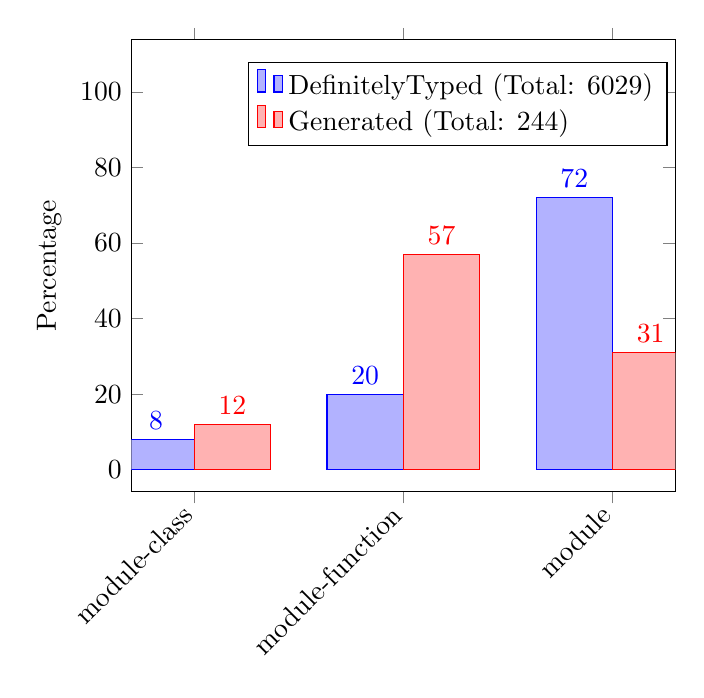
\begin{tikzpicture}
		\begin{axis}[
			ybar,
			width=0.7\textwidth,
			ybar=0pt,
			ymax=100,
			enlargelimits=0.15,
			bar width=0.08\textwidth,
			legend columns=1,
			legend cell align={left},
			legend style={at={(0.6,0.95)}, anchor=north},
			symbolic x coords={module-class,module-function,module},
			xtick=data,
			ylabel=Percentage,
			nodes near coords, 
			nodes near coords align={vertical},
			x tick label style={rotate=45,anchor=east},
		]
		\addplot coordinates {
			(module-class, 8)
			(module-function, 20)
			(module, 72)
		};

		\addplot coordinates {
			(module-class, 12)
			(module-function, 57)
			(module, 31)
		};
		\legend{DefinitelyTyped (Total: 6029), Generated (Total: 244)}
		\end{axis}
	\end{tikzpicture}

	\caption[TypeScript templates distribution | Generated \& DefinitelyTyped]{\textbf{TypeScript templates distribution | Generated \& DefinitelyTyped} - Out of a total of 6029, 72\% of the modules uploaded to the DefinitelyTyped repository use the \mintinline{text}{module} template and only 20\% use the \mintinline{text}{module-function} one. However, 57\% of the 244 generated declaration files use the \mintinline{text}{module-function} template.
	}

	\label{fig:experiments-typescript-templates-distribution-definitely-typed}
\end{figure}